\documentclass[twoside,a4paper,UKenglish,12pt]{report}     %% ... or USenglish or norsk or nynorsk

\usepackage[utf8]{inputenc}         %% ... or utf8 or applemac
\usepackage[T1]{fontenc,url}
\urlstyle{sf}
\usepackage{babel,textcomp,csquotes,duomasterforside,varioref,graphicx,hyperref,xcolor,longtable}
\usepackage[backend=biber,style=numeric-comp]{biblatex}
\usepackage[toc,page,title]{appendix}
\usepackage[nonumberlist,acronym,nomain]{glossaries}
%\usepackage{tabularx}

\usepackage{subcaption}
\captionsetup{font=small}
\captionsetup[sub]{font=scriptsize,belowskip=2pt,aboveskip=3pt}

\usepackage{mathtools}
\DeclarePairedDelimiter{\ceil}{\lceil}{\rceil}

\usepackage{tikz, floatrow, pgfplots, enumitem, mathtools, amsmath, bm}
\usetikzlibrary{positioning, shapes}

\newfloatcommand{capbtabbox}{table}[][\FBwidth]

\hypersetup{
  colorlinks,
  linkcolor={red!50!black},
  citecolor={blue!50!black},
  urlcolor={blue!80!black}
}

\usepackage[inner=3.5cm, outer=2.5cm, a4paper]{geometry} %% if not enough materials, change outer to 4.5
%\usepackage{showframe}
\usepackage{lipsum}

\title{Estimating Human pose from depth images using Convolutional Neural Networks}        %% ... or whatever
\subtitle{When all you got is a powerful GPU, everything looks like a CNN problem}         %% ... if any
\author{Bård-Kristian Krohg}                      %% ... or whoever 

\addbibresource{bib/sources.bib}                  %% ... or whatever
%% \addbibresource{bib/datasets.bib}
%% \addbibresource{bib/articles.bib}
%% \addbibresource{bib/papers.bib}
%% \addbibresource{bib/software.bib}
%%\addbibresource{sources.bib}
%%\bibstyle{plain}

\makeatletter
%%% ------- front, main and backmatter
\newcommand\frontmatter{%
    \cleardoublepage
  %\@mainmatterfalse
  \pagenumbering{roman}}

\newcommand\mainmatter{%
    \cleardoublepage
 % \@mainmattertrue
  \pagenumbering{arabic}}

\newcommand\backmatter{%
  \if@openright
    \cleardoublepage
  \else
    \clearpage
  \fi
 % \@mainmatterfalse
   }

%%% ------ big cdot for pretty dot products
\newcommand*{\bigcdot}{}% Check if undefined
\DeclareRobustCommand*{\bigcdot}{%
  \mathbin{\mathpalette\bigcdot@{}}%
}
\newcommand*{\bigcdot@scalefactor}{.5}
\newcommand*{\bigcdot@widthfactor}{1.15}
\newcommand*{\bigcdot@}[2]{%
  % #1: math style
  % #2: unused
  \sbox0{$#1\vcenter{}$}% math axis
  \sbox2{$#1\cdot\m@th$}%
  \hbox to \bigcdot@widthfactor\wd2{%
    \hfil
    \raise\ht0\hbox{%
      \scalebox{\bigcdot@scalefactor}{%
        \lower\ht0\hbox{$#1\bullet\m@th$}%
      }%
    }%
    \hfil
  }%
}
\makeatother
  % special command definitions

%%%%%%%%%%%%%%%%%%%     ACRONYMS      %%%%%%%%%%%%%%%%%%%

\newacronym{hri}{HRI}{Human Robot Interaction}
\newacronym{mecs}{MECS}{Multimodal Elderly Care System}
\newacronym{tof}{ToF}{Time-of-Flight}
\newacronym{har}{HAR}{Human Activity Recognition}
\newacronym{hpe}{HPE}{Human Pose Estimation}
\newacronym{ros}{ROS}{Robotic Operating System}
\newacronym{paf}{PAF}{Part Affinity Field}
\newacronym{roi}{RoI}{Region of Interest}

% computer vision
%% \newacronym{slam}{SLAM}{Simultaneous Localization and Mapping}
%% \newacronym{fast}{FAST}{Features from accelerated segment test}
%% \newacronym{brief}{BRIEF}{Binary Robust Independent Elementary Features}
%% \newacronym{orb}{ORB}{Oriented FAST and rotated BRIEF}
%% \newacronym{sift}{SIFT}{Scale Invariant Feature Transform}
%% \newacronym{surf}{SURF}{Speeded Up Robust Features}

%% \newacronym{ny}{NY}{New York}
%% \newacronym{la}{LA}{Los Angeles}
%% \newacronym{un}{UN}{United Nations}



%%%%%%%%%%%%%%%%%%%    NOMENCLATURE     %%%%%%%%%%%%%%%%%%%

%%%%%%    DEFINITIONS:
\newglossary{definition}{def}{dfn}{Glossaries}

\newglossaryentry{rgb}{
        type = definition,
        name = RGB,
        description = {Three channel image containing red, green and blue color information.},
        first = RGB
}

\newglossaryentry{rgbd}{
        type = definition,
        name = RGB-D,
        description = {Composite of a three channel RGB image, and an additional depth-channel containing the depth information in each pixel. Often, the depth channel is captured with a separate camera, and needs an additional calibration matrix to map the (u,v) pixel positions between the RGB channels and the depth channel.},
        first = RGB-D
}

\newglossaryentry{cnn}{
        type = definition,
        name = CNN,
        description = {A type of neural network that uses convolved filters to create spacial recognition more robust},
        first = CNN
}

\newglossaryentry{visual_hull}{
        type = definition,
        name = visual hull,
        description = {The 3D geometric volume occluded by a foreground object. The visual hull of an object is the 3D geometric volume produced behind the object when }
}


%%%%%%    SYMBOLS:
\newglossary{symbol}{sym}{sbl}{List of Symbols}

%% \newglossaryentry{sigma}{
%%         type = {symbol},
%%         name = {$\sigma$},
%%         sort = {sigma},
%%         description = {Surface tension}
%% }

\newglossaryentry{sol}{
        type = {symbol},
        name = {$c$},
        sort = {c},
        description = {Speed of Light}
}

%% \newglossaryentry{Mw}{
%%         type = {symbol},
%%         name = {$M_w$},
%%         sort = {Mw},
%%         description = {Molar mass}
%% }



%% \newglossaryentry{angelsperarea}{
%%   name = $a$ ,
%%   description = The number of angels per unit area,
%% }
%% \newglossaryentry{numofangels}{
%%   name = $N$ ,
%%   description = The number of angels per needle point
%% }
%% \newglossaryentry{areaofneedle}{
%%   name = $A$ ,
%%   description = The area of the needle point
%% }

\glsdisablehyper       % disable hyperlinks to glossaries
\makeglossaries

\begin{document}
\duoforside[dept={Institute for informatics},
  program={Informatics: Robotics and Intelligent Systems},
  long,
  printer={X-press printing house}
  %% image={img/vitruvian.png}
]{}
%% 悟 - enlightenment, percieve
%% 徴 - indication, sign, symptom
\frontmatter
\maketitle{}

\chapter*{Abstract}


This work is part of a larger project where we explore bringing robotics into geriatric
care. The goal of this project is to create a robotic system that can assist in optimizing
the use of physical personell, so they are used where they are needed.

This work will focus on capturing information about the user, anonymization of the data,
what data is neccessary or ethical to capture, limitations for on-location data processing
and what data can be sent for further processing in the cloud, or for human analysis.

We will also implement an ethical data-collection suite for the open-source Robotic
Operating System, which can be implemented on a wide variety of robots.

Convolutional Neural Networks has been used for solving object recognition in 2D images
with great success. This work aims to use the same techniques to extract 3D human pose
from depth images in real time. We will use two multi-staged CNNs, one to encode the
location of each joint, and another to encode the association between the joints to do this.

%% \begin{itemize}
%% \item what is it about (problem)
%% \item what has been done to ready the problem (method, data)
%% \item findings (main findings)
%% \item precautions for the findings
%% \item conclusion
%% \item implications
%% \end{itemize}


%% We look at novel ideas for detecting human pose in three dimensions for use in human activity recognition in geriatric care. We explore using convolutional neural networks directly on depth maps or indirectly, by transfering 2D pose found in complementary rgb images, and extrapolating the 3D joint locations.

                  %% ... or Sammendrag or Samandrag
\chapter*{Preface}
First, I would like to thank my supervisors Jim Tørresen and Ryo Kurazume, for their support, guidance, and patience during the development of this project. Second, my HR manager Marit Flendstad Kruse, for her assistance in letting me combine work with the writing of this thesis. Last, I would like to thank everyone at the Kurazume-lab for their welcome and help during my stay at Kyushu University, and my friends and family for proofreading and encouragement.

The subtitle, Both Eyes Open, has a double meaning: In this paper, we will explore the world in 3D. The biological way to achieve depth vision is by using two eyes, hence both eyes open. The other way to interpret the subtitle is tied with the small figure on the front page. In Japanese, the saying translated as "Both Eyes Open" refers to the Daruma figure. 

When one is working toward a goal, such as completing a thesis, one can purchase a Daruma figure from a temple. When bought, the Daruma has blank eyes - they are closed. The buyer then paints in one eye, asking for the Darumas help in completing their goal. In exchange for the Darumas help, the buyer promises to paint in the other eye. One significant detail about the Daruma is that it is weighted on the bottom.  If it should ever falter and fall over, it will right itself back up and continue on its way to completing the goal.

The ability to right yourself up for every setback has been of particular inspiration to me during my work on this thesis. This is why I have placed the figure on the front page; as a personal helper.


                   %% ... or Forord

\tableofcontents{}
\listoffigures{}
\listoftables{}

%% \input{tex/decl_acronyms}
%% \printacronyms[include-classes=abbrev, name=Abbreviations]{}
%% \printacronyms[include-classes=nomencl, name=Nomenclature]{}


\mainmatter

%%\part{Introduction}                   %% ... or Innledning or Innleiing
\chapter{Introduction}

%% Why collecting human pose
%% General introduction to this project
%% Three indentation layers is unneccessary
Finding human pose can have many applications inside the field of \gls{hri}, to understand the intent of a person, if they are aware of the robot, their position in relation to the robot, help understand their reaction to an interaction via body-language, or the action the person is doing at any one time.

Human pose can also help professionals understand a patient better. If tracked over time, we can see changes in the persons gait, their posture or track their daily activities. All this can be used to asess if treatments are working or come up with changes in a persons activity schedule.


What we \textit{say} can say a lot. However, some may argue that our body language, says even \textit{more}. Our pose is a. It can say something about our emotional state, physical state, or it could say something about our intention or activity in a moment in time. Sequences of poses can give us an even better idea about actions and activities. A still pose can have us guessing at what a person is doing, however if we have a sequence of poses, we can know for \textit{sure}. Given a sequence of poses, we can distinguish between a person just slav-squatting, or if they are putting some real effort into a frog-jump. We can also probably recognize if a person is going to fall over, or if they're just walking normally.




\section{Human Pose Estimation}
For The \gls{mecs} to function as intended, it is imperative that it can detect humans reliably. And for \gls{har} we need accurate pose estimation.

\section{Multimodal Elderly Care System}
\subsection{Motivation}
As life expectancy increases in Norway, so does the population who needs geriatric care either at home, or in a geriatric facility. Accodring to \cite{oslohelsa}, it is projected that mainly the elderly population in Oslo will increase in the coming years, and that this will lead to increased pressure on the healthcare services.

As part of the effort to let people live independently at home for as long as possible, we propose a \gls{mecs}. One of the goals for the \gls{mecs} is to function as an autonomous safety alarm, a device that lets elderly living at home call the emergency services at the click of a button. However, if the emergency is an accident which renders the user incapacitated, or otherwise unconscious, an alarm that requires interaction will not be of much help. In contrast, the \gls{mecs} can monitor a user, and warn healthcare personnel in case of an occuring, or predicted, emergency. The \gls{mecs} will even be able to send contextual information to first-responders, which lets them better prepare for the situation.

We also strive to make the system non-invasive, as this will increase the convenience for the user, in that the \gls{mecs} will not require any interaction from the user to function. Taking the user out of the operational loop has many other advantages as well. For example, a monitoring system in the form of a smartwatch, will be inconvenient and ineffective the user forgets to put it on.

Further, it is hypothesized that the information gathered by the \gls{mecs} can help doctors or physical therapists prescribe or recommend health-promoting activities for the user. This could help prevent accidents or lifestyle diseases -- which again will help relieve pressure on the communal healthcare services.

\subsection{Hardware}
The \gls{mecs} is envisioned to be a small, mobile unit as this can be introduced to any home without extensive alterations to the environment, thus lowering the cost of the system and reusability of the units. As the \gls{mecs} would need a charging station anyway, we propose a master/slave configuration between a stationary and a mobile unit, which should communicate through a secure wireless connection, for example a WLAN. We let the stationary unit take care of the power consuming complex processing, extending the operational time for the mobile unit between battery charges. We will therefore assume the system has access to mid- to high-end personal GPU/processing hardware, when we evaluate the real world practicality/runtime of the algorithm.

To provide as good a service for the user as possible, we believe that gathering many channels of information will be helpful. We wish to learn the users daily activity patterns or vital signs so when unhealthy or risk-filled patterns emerge, preventative actions can be implemented. \gls{har}, gate/mood recognition, or detection of vital signs all require us to know where the user is in the scene.

This also places some requirements on our system. If the system solely relies on this work to find humans in the scene, we set our lower framerate limit to 8 fps to be able to preform human heart rate aquisition~\cite{Wu12Eulerian}\footnote{If the maximum human heart rate is 220 bpm, and we want to measure it accuratley using video sequences produced by the \gls{mecs}, our sampling frequency needs to be higher than $7.\overline{3}$ Hz in order to satisfy the Nyquist rate.}. Further, the \gls{mecs} needs to be able to recognize humans in unstructured environments, in a variety of poses and to diffrentiate between multiple people.

In order to log the users activity patterns, and detect anomalies or deviations in this, we envision the \gls{mecs} doing \gls{har}.

\subsection{Privacy}
%% TODO: first draft -- rewrite!!!
The information gathered by this system should only be available to the users designated doctors/physisians and to the user themselves, and should be treated at the same classification level as any persons medical journal. This means that the dataprocessing from the \gls{mecs} must happen on-site, or that any cloud processing happens under a user agreement that protects this data from those owning the servers. The same agreement should count for anyone making the hardware/software that is used in the \gls{mecs}.

The \gls{mecs} is also capable of gathering additional data that is not relevant for the healthcare personell. For example, by using depth sensors we are able to create 3d maps of the users home or environment. this is helpful for the \gls{mecs}, however it is not relevant for the healthcare personel. (with the exception of first responders, which could get the information either through a descriptive message -- ``the patient is in the bathroom on the second floor, no elevator, steep stairs'' or via the actual internal map the \gls{mecs} has created for its own internal navigation.)


\chapter{Background}

\section{Convolutional Neural Networks}



\section{Pose Estimation}
In this work we are heavily inspired by \cite{cao2017realtime} that uses two convolutional neural networks to find human pose. One of the networks finds the probability for the 2D location of a set of joints, we get $N$ confidence maps for the locations of each $N$ number of joints. The other creates $M$ \gls{paf} the probability maps for $M$ number of limbs\footnote{In this work we'll stick to the convention of using the term limb to describe any connection between any pair of body landmarks, which we call joints.}. We then use the results from this \gls{paf} to find out which joints from the first result should be connected.
\begin{figure}[h]
  \begin{subfigure}[t]{0.24\textwidth}
    \includegraphics[width=1\linewidth]{img/openpose_pipeline_a}
    \label{fig:oppA}
    \caption{Input Image}
  \end{subfigure}%
  ~
  \begin{subfigure}[b]{0.24\textwidth}
    \begin{subfigure}{1\textwidth}
      \includegraphics[width=1\linewidth]{img/openpose_pipeline_b}
      \label{fig:oppB}
      \caption{Part Confidence Maps}
    \end{subfigure}
    
    \begin{subfigure}{1\textwidth}
      \includegraphics[width=1\linewidth]{img/openpose_pipeline_c}
      \label{fig:oppC}
      \caption{Part Affinity Fields}
    \end{subfigure}
  \end{subfigure}%
  ~
  \begin{subfigure}[t]{0.24\textwidth}
    \includegraphics[width=1\linewidth]{img/openpose_pipeline_d}
    \label{fig:oppD}
    \caption{Bipartite Matching}
  \end{subfigure}%
  ~
  \begin{subfigure}[t]{0.24\textwidth}
    \includegraphics[width=1\linewidth]{img/openpose_pipeline_e}
    \label{fig:oppE}
    \caption{Parsing Results}
  \end{subfigure}
  \caption{The pipeline described in \cite{cao2017realtime}. The input image \ref{fig:oppA} is fed into the two networks which produce joint detections in confidence maps \ref{fig:oppB} and \gls{paf}s \ref{fig:oppC}. They then preform bipartite matching in \ref{fig:oppD} to determine which detected joints should be connected by a limb. \ref{fig:oppE} shows the finished results.}
\end{figure}

Using the method described in \cite{cao2017realtime} we however don't get any information if some pairs of joints are missing, for example due to occlusion or failure to detect the body landmark, leading to an incomplete skeleton.


A lot of research\footnote{TODO: Cite Research} has been going into extracting human pose either from RGB images, or using depth images. Although many methods exists such as \emph{Histogram of Gradients (HoG)} classifiers,

A lot of research has been done in estimating human pose in two dimensions, as this is where we have quite large datasets, such as the MPII, or the Human 3.6M datasets \cite{andriluka14cvpr,h36m_pami}.

\textbf{Background extraction}

\textbf{HoG classifiers}


\textbf{Motivation for 3D pose} To train any network using supervised learning, we need large amounts of training data. One of the goals for the MECS project is to do \emph{Human Activity Recognition (HAR)}, so one can track the user from day to day and look for patterns that could lead to worsening living conditions. We also want to be able to recognize the activity from any viewpoint, and this is where a 2D approach will lack robustness. This is because any HAR model trained solely on 2D data, will only be able to recognize the activity from the views it has seen the activity being preformed. A 3D approach will provide us with robustness in respect to view-independentness.




%% {\color{red}\textbf{TODO REMOVE:\newline Just some stuff with \gls{sigma} and \gls{Mw}. and \gls{rgb} and \gls{rgbd} jsut to test and also Thomas Simon~et~al.~\cite{simon2017hand} showed that we won't actually ues this reference.}}

%% \chapter{Earlier work}
%% \lipsum

%% \chapter{Planning the project}        %% ... or ??
\chapter{DepthPose}
%% WHAT IS IMPLEMETED
%% WHY DOES IT REPRESENT A PROGRESS IN RESEARCH

%% Objective of the system
The DepthPose here introduced is a complete system for extracting human 3D poses from a single depth image in real-time\footnote{Real-time is defined as being capable of processing at least 30 depth frames per second on the specified minimum hardware requirements.}. It is specifically tailored for use in robotic applications where computational resources are limited. Because the \gls{mecs} is envisioned to be a mobile unit, DepthPose has to be robust to be able to see the person from different viewing angles despite possible occlusions between the person and the depth-sensor. The architecture is inspired by and builds on the architecture in OpenPose~\cite{cao2019openpose}. The general pipeline of DepthPose follows the OpenPose pipeline in figure~\ref{fig:openpose_pipeline} closely, with the addition of a novel Articulation Network that refines the poses after the bipartite matching.

%% Why 3D?
One of the goals for the \gls{mecs} project is to look for patterns that could lead to worsening or more dangerous living conditions. To that end, \gls{har} is implemented with the purpose of tracking a user from day to day. Representing the pose in 3D will simplify application areas such as \gls{har}, because a 3D representation of a skeleton can be defined by a coordinate system constrained to any two connected limbs from the observed skeletons. This means that two different skeleton observations can be represented by a common reference point. Had the skeletons been represented in 2D, the same skeleton seen from two different angles could look vastly different, even if referenced from the same limb. Comparing the two 2D poses will therefore be a more difficult problem than comparing the same poses referenced from a common 3D coordinate system.

%% TODO> about not needing a full 3D body mesh, and privacy concerns


\section{Architecture}

The system pipeline is outlined in figure~\ref{fig:arch_main}. As in \cite{cao2019openpose}, two stages are used to extract the pose from an image. In each stage, a \gls{rnn} architecture iteratively refines the output from the network at that stage. This iterative architecture was inspired by Convolutional Pose Machines~\cite{wei2016cpm}.

At timestep $t = 0$ in the first stage, a set of depth features are created by the first \gls{cnn}, $df$. These are stacked with the \emph{limb-maps} produced by the next \gls{cnn}, $lp$. At $t = 0$ these limb-maps will be initialized to a known value, \textbf{0}, so only the learned bias weights influence $lp$ at this timestep. $lp$ will then refine these limb-maps at subsequent timesteps $0 < t \leq T_{P}$.

At timestep $t = T_{P} + 1$ the refined ``first guess'' limb-maps from $lp$ are again stacked with the depth features from $df$, and used as inputs to $jp$ which produces a set of likely \emph{joint-maps}. These joint-maps are then passed to the Assembly function, which performs the bipartite matching algorithm and constructs a set of skeletons. An instance of the Articulation Network is created for each of the detected skeletons. The Articulation Networks refine the poses for each of the detected skeletons. The refined skeleton poses are then projected onto a set of limb-maps which is used instead of the ``first guess'' limb-maps from $lp$, in successive timesteps $T_{P} + 1 < t \leq T_{P} + T_{C}$.

%% As in \cite{cao209openpose}, two networks are used to create the \gls{paf}s and the confidence maps for the joints. However, instead of training on 3-channel RGB images, we will use a single channel depth image to discover the body landmarks/joints.
%% However, since depth images are single channel, and thus have less information than the RGB images, we propose using a shallower network. This also means we have to do the first step of feature extraction which was already done in a
%% However, since the depth images are less detailed than normal RGB images, some landmarks might be harder to detect: eyes, nose, or placing the joint on an outstretched limb.

%% TODO> about shallowness of network

%% The architecture of this project is \emph{recurrent} in that it repeats itself for a number of iterations. As with the architecture in \cite{cao2017realtime}, we have to have a first step which produces the first outputs we can use in later steps. However, this step is not illustrated in Fig.\ref{fig:arch_main}, since the first step will be identical to the next steps, except it will not have the additional inputs produced by the outputs of the previous step.

\begin{figure}[h]
  \centering
  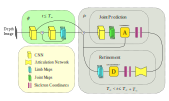
\includegraphics[width=\textwidth]{img/architecture_main}
  \caption[Main architecture]{Main architecture, as in \cite{cao2017realtime} two recurrent stages, $\phi^{t}$ and $\rho^{t}$ are used to iteratively refine the limb and joint locations.}
  \label{fig:arch_main}
\end{figure}

\subsection{Depth feature extraction}\label{subsec:depth_feature}

\begin{figure}[h]
  \centering
  \includegraphics[width=.9\textwidth]{img/rgbd_example}
  \caption[RGB-D Example]{Example of an RGB image on the left vs. a comparative depth image of the same scene on the right. Excerpt sourced from \cite{phdthesisMaxime}.}
  \label{fig:rgbdex}
\end{figure}

The main task for the \gls{cnn} $df$ is to find useful depth features for the subsequent networks. As illustrated in Figure~\ref{fig:rgbdex}, the information in depth images is not as dense as in RGB images. With the goal of object recognition, networks that are trained on RGB images could rely on features such as colors and textures. For example, the blue shirt vs. the khaki pants or the checkerboard pattern of the floor. However, none of those features are present in the depth image. In both images, edges could be extracted to indicate the outline of objects. Indeed, the edges detected in the depth image could be more useful for this purpose than in the RGB image because they would represent the actual 3D boundary between two objects. A quick example could be two boxes of the same color placed partly behind each other. In an RGB image, they could appear to be part of the same object, whereas a sharp edge would separate them in a depth image. Still, much of the information in depth images have to rely on gradients and other features at a larger scale. It can be speculated that representations for planes geometric or organic shapes will be learned.

Figure~\ref{fig:point_cloud} shows that depth images can also be represented as points in a volume. However, to use such a representation of the data as input to a 3D \gls{cnn}, a limit would have to be placed on the observed depth to define a fixed input size. This would lead to a sparse representation of the data, where many convolutions would contain empty space. Since no information can be gathered in the occluded parts of the scene anyway, a single channel depth image is a more succinct representation of the input.

As discussed in Section~\ref{sec:background_cnn}, the feature extraction parts of a network can be trained on large, unrelated datasets. However, no models that were pre-trained on depth images were found, so applying transfer learning for this part of the network was not an option. This part of the model is therefore not necessarily optimal, and having only seen the inside of a dome, it might not have found features that would perform better in a real-world environment.

\begin{figure}[h]
  \centering
  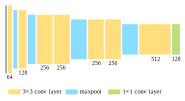
\includegraphics[width=.7\textwidth]{img/convvgg}
  \caption[Depth Feature Extraction]{Depth feature extractor network. The maxpool layers has size $2 \times 2$ and stride 2. Each convolutional layer uses the \gls{relu} activation function.}
  \label{fig:depth_feature_network}
\end{figure}

The OpenPose architecture reuses the first 10 layers of VGG-19 (E configuration)~\cite{simonyan2015deep}. Therefore, this part of the network takes inspiration from it as well. VGG-19 is constructed using several $3 \times 3$ convolutional layers with \gls{relu}~\cite{nairHintonRelu} activations, and maxpool operations at certain depths. By only using enough $3 \times 3$ convolutional layers, the number of learnable parameters are kept down, while preserving the receptive field of a larger kernel (not stacked)\footnote{For an input and output consisting of two channels the learnable parameters can calculated: One $7 \times 7$ kernel $\rightarrow 7^{2}C^{2} = 49C^{2}$ parameters. Three stacked $3 \times 3$ kernels $\rightarrow 3(3^{2}C^{2}) = 27C^{2}$ parameters.}. This is ideal for keeping the network as small, and thus as fast as possible. However, since the information at a small scale can be sparse in depth images, dilation is used to obtain a larger receptive field for each convolutional layer. This is different from pooling layers, because they emit which \emph{feature} in a certain layer has the strongest, weakest or calculate what the average response to the input was. On the other hand, a dilated convolutional layer \emph{creates} features for a larger receptive field, and does not downscale the spacial dimensions of the feature tensor, if same-padding is utilized. The first convolutional layer in Figure~\ref{fig:depth_feature_network} uses dilation of 4 to compensate for the lack of small-scale features in the depth image.

%% \begin{table}
%%   \centering
%%   \begin{tabular}[h]{|c|c|}
%%     \hline
%%     Depth Features $df$ & Limb/Joint Maps $lp$/$jp$ \\
%%     \hline
%%     \hline
%%     Depth image & Features+$lm$ \\ \hline
%%     conv3-64 & conv3 \\ \hline
%%     maxpool & conv3 \\ \hline
%%     conv3-128 & conv3 \\ \hline
%%     maxpool & conv3 \\ \hline
%%     conv3-256 & conv3 \\ \hline
%%     conv3-256 & conv3 \\ \hline
%%     maxpool & conv3 \\ \hline
%%     conv3-256 & conv3 \\ \hline
%%     conv3-256 & conv3 \\ \hline
%%     maxpool & conv3 \\ \hline
%%     conv3-512 & conv3 \\ \hline
%%     conv3-512 & conv3 \\ \hline
%%     conv1-128 & conv3 \\ \hline
%%   \end{tabular}
%%   \caption{\gls{cnn}s presented in this work. \gls{relu}s are omitted for brevity.}
%%   \label{tab:cnns}
%% \end{table}

\begin{figure}[h]
  \centering
  \includegraphics[width=.7\textwidth]{img/depth_image_receptive_fields}
  \caption[Receptive fields in depth images]{Relevant receptive fields in a depth image. Fields are shown as green boxes, with sizes placed near the edge.}
  \label{fig:depth_fields}
\end{figure}

\subsection{Limb- and Joint-Maps}

In \cite{cao2019openpose,wei2016cpm} it is observed that the receptive field of the convolutions are important to establish long-range inferences about body landmarks. This might be because the network learns about the natural symmetries in the human body, and can therefore more easily predict the relationship between different body parts.

In the revisited version of OpenPose, the $7 \times 7$ convolution blocks in the pipeline are replaced by convolution blocks of three $3 \times 3$ filters, where the emissions from each filter is concatenated at the end of the block. This preserves the receptive field of the convolution block, while reducing the number of learnable parameters, as noted in \cite{simonyan2015deep}. In addition, by concatenating the result from each layer at the end of the block, a type of residual network~\cite{he2015deep} is created, mitigating the vanishing gradient problem.

DepthPose uses three such convolution blocks, with a two final $1 \times 1$ convolution layers with dropout between them. This final feature vector is then upsampled through a transposed convolution layer. The output of this is a tensor of $w \times h \times N$ where $N$ is the number of feature maps needed for the network. Since the limb and joint maps look for the same kind of long-reaching features, the architecture is similar.

The limb-map network produce tensors $3M \times w \times h$ where $M$ is the number of limbs in a skeleton. Each limb has 3 components, as they encode the vector pointing in the direction of the limb at that coordinate.

The joint-maps are tensors $2N \times w \times h$ where $N$ is the number of joints in a skeleton. The tensors encode the depth of the limb at that location, as well as the confidence.

%% For each pixel in the current layer of the \gls{cnn}, we collect information from a filter-sized portion of the previous layer. This means that deeper layers look at a larger and larger portion of the input layer. This is useful for detecting connections between large-scale structures. This also means that after a certain depth, there may not be any more useful information.

%% In our experiments, we will try different depths for feature extraction.

%% Some of these features might be desirable as inputs for later layers in object classification.

%% This network is built from the ground up. Therefore we want some layers to, for example, detect edges and one for detecting slanting gradients or connected surfaces. For limbs, we might want to find surfaces that are shaped like tubes or oblong spheroids.

\subsection{Articulation network}\label{subsec:articulation}
The articulation network solves the problem where two people occludes the other. If a joint of the same body part for two people is co-linear to the camera, this joint can not be represented in the joint-map for the occluded person.

The articulation network is stacked on top of the part-detection network and its main role is to refine the limb lengths and angles between each joint. Each of the detected persons are passed through the articulation network, which leads to a bit more complexity and runtime for the network based on the number of people. However, since the network has so comparatively few inputs, and is quite shallow, preformance is not expected to suffer notably.

The coordinates and confidences for each joint (if not detected, confidence is 0) is the input to the network. The network will try to find out what the positions of joints with low confidences, or no detections, should be. It is hypothesized that this network will learn things like symmetry (left and right limbs should have the same length), proportionality (limbs should be proportional to each other), possible articulations, and natural poses.

The architecture is visualized as a simple, almost fully connected neural network. Since each joint has four properties, (x, y, z, c), these are input to a single neuron in the network. The layers after this is however fully connected.

\section{Assembly}

Done in the same way as \cite{cao2019openpose}, however the score-equation for the line integral is
\begin{equation}
  S = \sum_{i=0}^{K}\cos(\theta)
\end{equation}
$\theta$ is the angle between the the vector defined by the candidate points and the angle of the vector at the points of the limb-maps along the line $i, K$

\begin{figure}[h]

  \begin{floatrow}
    \ffigbox{
      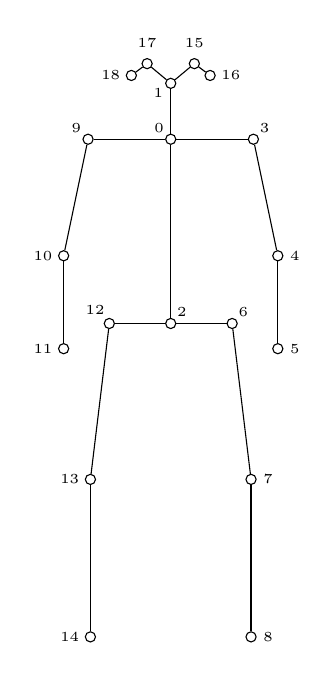
\begin{tikzpicture}[
          every node/.style={draw,circle,minimum size=.06cm, inner sep=1.3pt}
        ]
        \tiny
        %% \draw[help lines, step=5mm, gray!20] (-4,-4) grid (3,4);
        %% Standard coordinates => (orig.coords) - (0, .2)
        \node[label={[label distance=-.2mm]140:{0}}] (neck) at (0,2.54) {};
        \node[label={[label distance=-.2mm]200:{1}}] (nose) at (0,3.25) {};
        \node[label={[label distance=-.2mm]50:{2}}] (mhip) at (0, .2) {};

        \node[label={[label distance=-.2mm]50:{3}}] (lshoulder) at (1.05,2.54) {};
        \node[label={[label distance=-.1mm]0:{4}}] (lelbow) at (1.36,1.06) {};
        \node[label={[label distance=-.1mm]0:{5}}] (lwrist) at (1.36,-.12) {};
        \node[label={[label distance=-.2mm]50:{6}}] (lhip) at (.78,.2) {};
        \node[label={[label distance=-.1mm]0:{7}}] (lknee) at (1.02,-1.78) {};
        \node[label={[label distance=-.1mm]0:{8}}] (lankle) at (1.02,-3.78) {};

        \node[label={[label distance=-.2mm]140:{9}}] (rshoulder) at (-1.05,2.54) {};
        \node[label={[label distance=-.1mm]180:{10}}] (relbow) at (-1.36,1.06) {};
        \node[label={[label distance=-.1mm]180:{11}}] (rwrist) at (-1.36,-.12) {};
        \node[label={[label distance=-.2mm]140:{12}}] (rhip) at (-.78,.2) {};
        \node[label={[label distance=-.1mm]180:{13}}] (rknee) at (-1.02,-1.78) {};
        \node[label={[label distance=-.1mm]180:{14}}] (rankle) at (-1.02,-3.78) {};

        \node[label={[label distance=-.1mm]90:{15}}] (leye) at (.3,3.5) {};
        \node[label={[label distance=-.1mm]0:{16}}] (lear) at (.5,3.35) {};
        
        \node[label={[label distance=-.1mm]90:{17}}] (reye) at (-.3,3.5) {};
        \node[label={[label distance=-.1mm]180:{18}}] (rear) at (-.5,3.35) {};

        %% \draw[blue] (0,0) circle [radius=.06cm];

        \draw (nose) -- (neck);
        \draw (neck) -- (mhip);

        \draw (reye) -- (nose); \draw (leye) -- (nose);
        \draw (reye) -- (rear); \draw (leye) -- (lear);
        
        \draw (neck) -- (rshoulder); \draw (neck) -- (lshoulder);
        %% \draw (neck) -- (rhip); \draw (neck) -- (lhip);
        \draw (neck) -- (mhip);

        \draw (rshoulder) -- (relbow); \draw (lshoulder) -- (lelbow);
        \draw (rwrist) -- (relbow); \draw (lwrist) -- (lelbow);

        \draw (mhip) -- (rhip); \draw (mhip) -- (lhip);
        \draw (rhip) -- (rknee); \draw (lhip) -- (lknee);
        \draw (rknee) -- (rankle); \draw (lknee) -- (lankle);
      \end{tikzpicture}
    }
    {
      \caption[Numbering for keypoint markers]{Numbering for detected landmarks/keypoint markers.}
      \label{fig:skeleton_markers}
    }
    %% \end{figure}
    %% \begin{table}
    \capbtabbox{
      \footnotesize
      \begin{tabular}[H]{|r l r|}
        \hline
        \textbf{ID} & \textbf{Description} & \textbf{Std.Coord.} \\ \hline
        0  & Neck & (0.00, 2.34) \\
        1  & Nose & (0.00, 3.05) \\
        2  & Middle hip & (0.00, 0.00) \\
        3  & Left shoulder & (1.05, 2.34) \\
        4  & Left elbow & (1.36, 0.86) \\
        5  & Left wrist & (1.36, -0.32) \\
        6 & Left hip & (0.78, 0.00) \\
        7 & Left knee & (1.02, -1.98) \\
        8 & Left ankle & (1.02, -3.98) \\
        9  & Right shoulder & (-1.05, 2.34) \\
        10 & Right elbow & (-1.36, 0.86) \\
        11 & Right wrist & (-1.36, -0.32) \\
        12 & Right hip & (-0.78, 0.00) \\
        13 & Right knee & (-1.02, -1.98) \\
        14 & Right ankle & (-1.02, -3.98) \\
        15 & Left eye & (0.30, 3.30) \\
        16 & Left ear & (0.50, 3.15) \\
        17 & Right eye & (-0.30, 3.30) \\
        18 & Right ear & (-0.50, 3.15) \\
        \hline
      \end{tabular}
    }{
      \caption[Names/coordinates for detected landmarks]{Numberings, names/descriptions and standard coordinates for recognized landmarks}
      \label{tab:openpose_body_ids}
    }
  \end{floatrow}          
\end{figure}

\section{Training}
%% criterion, why was this chosen
%% Learning rate
%% optimizer




%% \section{2D detection transfer}

%% (First ideas.)

%% Torso placement and tree structure for placing.

%% Fit to human standard model (rules for symmetry and lengths)

%% Occlusion problem, and interpolated points, visual hull constraints

%% We train the network on both depth images and a kinematic model of each 3D ground truth location.

%% \section{Pose from CNN over depth maps}

%% We create a separate 'side-view' detection map for each 'frontal' detection map. This reduces the convolution operations, since we don't have to convolve over the whole 3D space.

%%\part{Implementation}
%% \chapter{The Project}

\section{Human Robot Interaction Package for ROS}

%% USE A DESCRIPRIVE TITLE! (ie. Robot Brain Implementation)
%% See your choises in birds eye perspective. how you can discuss what youve done.


%% What was made, why is it good. document all choices. The rule is that a different scientist with the same resources should be able to get the same results based on your description. Dont write about the methods in general, but exactly what youre doing. discuss your own approach. Show that youre aware there are other alternatives to what you did, and what advantages a different method may have. Did you have any influence over how things were solved. what is strengths and weaknesses about your work. what would you do different if you were to do it again? be open about weaknesses, but defend your choices. Refer to other researchers who has done the same. 

A multipurpose package for tracking information about humans was made. The package features both detection of 2D joints as well as a method of manually fitting a whole 3D skeleton to the observed points.

\section{Human Pose Estimation}

The robot we're developing needs to be able to robustly detect humans, so information about their state can be gathered and analyzed. To accomplish this task, we propose a system that uses RGB-D data in combination with IR images to estimate the 3D pose of humans. In addition we propose a manual algorithm for estimation of occluded parts that can not be directly observed. 

A lot of work has already been done on human pose estimation, however this approach focuses on creating a manual method for constraining the 3D skeleton and estimating the 3D pose of the observed person. We rely on 2D detection of joints for each person by the OpenPose software. 

\begin{figure}
  \centering
  \begin{floatrow}
    \ffigbox[.3\textwidth]{
      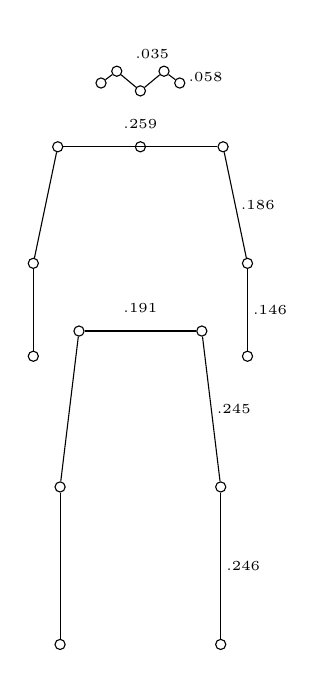
\begin{tikzpicture}[
          every node/.style={draw,circle,minimum size=.06cm, inner sep=1.3pt}
        ]
        \tiny
        %% \draw[help lines, step=5mm, gray!20] (-4,-4) grid (3,4);
        
        \node (nose) at (0,3.25) {};
        \node (neck) at (0,2.54) {};
        
        \node (reye) at (-.3,3.5) {};
        \node (leye) at (.3,3.5) {};

        \node (rear) at (-.5,3.35) {};
        \node (lear) at (.5,3.35) {};

        \node (rshoulder) at (-1.05,2.54) {};
        \node (lshoulder) at (1.05,2.54) {};
        
        \node (relbow) at (-1.36,1.06) {};
        \node (lelbow) at (1.36,1.06) {};

        \node (rwrist) at (-1.36,-.12) {};
        \node (lwrist) at (1.36,-.12) {};

        \node (rhip) at (-.78,.2) {};
        \node (lhip) at (.78,.2) {};

        \node (rknee) at (-1.02,-1.78) {};
        \node (lknee) at (1.02,-1.78) {};

        \node (rankle) at (-1.02,-3.78) {};
        \node (lankle) at (1.02,-3.78) {};

        %% \draw[blue] (0,0) circle [radius=.06cm];

        \draw (reye) -- (nose); \draw (leye) -- node[above, draw=none, inner sep=2.5pt] {.035} ++(nose);
        \draw (reye) -- (rear); \draw (leye) -- node[right, draw=none, inner sep=4.3pt] {.058} ++(lear);

        %% \draw (rear) -- node[below right, draw=none, xshift=5pt] {.105} ++(lear);
        
        \draw (lshoulder) -- node[above, draw=none] {.259} ++(rshoulder);

        \draw (rshoulder) -- (relbow); \draw (lshoulder) -- node[right, draw=none] {.186} ++(lelbow);
        \draw (rwrist) -- (relbow); \draw (lwrist) -- node[right, draw=none] {.146} ++(lelbow);

        \draw (rhip) -- (rknee); \draw (lhip) -- node[right, draw=none] {.245} ++(lknee);
        \draw (rknee) -- (rankle); \draw (lknee) -- node[right, draw=none] {.246} ++(lankle);

        \draw (rhip) -- node[above, draw=none] {.191} ++(lhip);
      \end{tikzpicture}
    }
    {
      \label{fig:constrained_lengths}
      \caption[Constrained Lenghts]{Constrained limb connections.}
    }
    %% \end{figure}
    %% \begin{table}
    \capbtabbox{
      \begin{tabular}[H]{|r l|l|c|}
        \hline
        ID & Limb & Model & Pair \\ %%& $\pm\bm{t}$ \\
        \hline
        0 & Left arm & .186 & 5 -- 6 \\ %% & .05 \\
        1 & Left forearm & .146 & 6 -- 7 \\ %%&.05 \\
        2 & Right arm & .186 & 2 -- 3 \\ %%& .05\\
        3 & Right forearm & .146 & 3 -- 4 \\ %%& .05\\
        4 & Hip & .191 & 8 -- 11 \\ %%& .06\\
        5 & Left thigh & .245 & 11 -- 12 \\ %%& .07 \\
        6 & Left leg & .246 & 12 -- 13 \\ %%& .07 \\
        7 & Right thigh & .245 & 8 -- 9 \\ %%& .07 \\
        8 & Right leg & .246 & 9 -- 10 \\ \hline %%& .07 \\ \hline
      %%   $\lvert Right shoulder - Right elbow\rvert = \lvert Left shoulder - Left elbow \rvert$
      %%   \hline
      \end{tabular}
    }{
      \label{tab:constrain_rules}
      \caption[Anthropometry constrain rules]{Constrain rules for correct anthropometry. (Note that the anthropometry for the head and shoulders are not yet implemented.)}
    }
  \end{floatrow}
\end{figure}

\subsection{Formulas for constraining}

For a fixed point $a$ we want to move a point $b$ so the Euclidean distance between them is equal to $L$. A few different methods was developed to accomplish this, based on the reliability of the different keypoints.

\subsubsection{Keypoint projection}
If both $\vec{a}$ and $\vec{b}$ are well-observed points and the initial distance between the point $\vec{a}$ and the line from the camera center through $\vec{b}$ are less than $L$, we use the following formula to calculate the new position of $\vec{b}$.
We get the length, $x$ of the vector to the new position of $\vec{b}$ by using equation~\ref{eq:pushvector}. The constrained point is then simply defined as $x|\vec{b}|$.
\begin{equation}
  x = \max\left(\frac{2(\vec{a} \boldsymbol{\cdot} \vec{b}) \pm \sqrt{4(\vec{a} \boldsymbol{\cdot} \vec{b})^{2} - 4 ||\vec{b}||^{2} (||\vec{a}||^{2} - L^{2})}}{2 (||\vec{a}||^{2} - L^{2})}\right)
  \label{eq:pushvector}
\end{equation}
However, if the minimum distance between $\vec{b}$ and the line is more than $L$, we define the point as the point $L$ away from point $\vec{a}$ on the line through the coordinates of $\vec{a}$ perpendicular to the line along $\vec{b}$. The point is then defined by equation~\ref{eq:perpendicular}.
\begin{equation}
  \vec{p} = \vec{a} + L\left|\vec{a} - \frac{\vec{a}\boldsymbol{\cdot}\vec{b}}{\vec{b}\boldsymbol{\cdot}\vec{b}} \boldsymbol{\cdot} \vec{b}\right|
  \label{eq:perpendicular}
\end{equation}

\subsubsection{Keypoint interpolation}
This method could be used both to create one additional keypoint, or to determine the location of an obstructed keypoint. We assume we again have two well observed keypoints $a$ and $c$. We wish to find the location of keypoint $b$.
To interpolate, we imagine two spheres around point $a$ and $c$ with radiuses $r_a, r_c$. The interpolated point must be on the intersecting circle between the two spheres. The distance from point $a$ to the plane of that circle is defined as $x = \frac{d^2 - r_c^2 + r_a^2}{2d}$ where $d$ is the Euclidean distance $||a - c||$. The radius of the circle is defined as $h = \frac{1}{d}\sqrt{(-d+r_c-r_a)(-d-r_c-r_a)(-d+r_c+r_a)(d+r_c+r_a)}$. The keypoint $b$ is then defined as the keypoint furthest away from the camera on this circle. In later versions this could be constrained by the angle between the previous limb and this one.

\subsection{Skeleton fitting}

We wish to fit a constrained skeleton to the observed points in 3D space. Our skeleton is defined as three separate graphs with constrained edges.
The keypoints defining the nodes of the graphs (joints) are detected by the OpenPose network, and sorted based on the confidence of detection. For each graph a subset of $n$ keypoints are picked as seeds, and constrained graphs are generated:\\
Scale (and thus limb length) is calculated based on the confidence of the keypoints using the weighted sum in equation~\ref{eq:scale} where $L$ is the set of Euclidean lengths in each graph and $S$ is the scores of those lengths. $S$ is calculated by the Gaussian function of the confidence of the scores $c_a$ and $c_b$ with $\sigma = 0.33$ as described in equation~\ref{eq:limb_score}.
\begin{equation}
  S = \frac{\sum_{i=0}^{N}L(i) \cdot s(i)}{\sum_{i=0}^{N}s(i)}
  \label{eq:scale}
\end{equation}
\begin{equation}
  s = \frac{1}{\sqrt{\sigma\pi}}e^{-\frac{1}{\sigma}(c_a-1)^2 + (c_b -1)^2}
  \label{eq:limb_score}
\end{equation}
    {\color{red} Alternative notation for equation~\ref{eq:limb_score} because of possible cumbersome notation in $e$ expression.
\[
s = \frac{1}{\sqrt{\sigma\pi}}{\exp}\left(-\frac{1}{\sigma}(c_a-1)^2 + (c_b -1)^2\right)
\]}
We then recursively constrain all points based on a seed point from the sorted keypoints. If no keypoints with confidence over a certain threshold $t$ are detected, the graph is not placed.
The constrained graph is moved to the center of the detected keypoint, again weighted by $S$, and we are finished constraining the graph.

The skeleton is defined as the subset of graphs best matching their respective keypoints where scale is similar.

%% \chapter{Experiments}                     %% ... or ??

{\color{red}What did we find out. dont overcomplicate the explanation. this could be the longest part of the thesis. about 15-20 pages? If you have more questions, use that as structure for this section. You can divide this into multiple chapters: subsidiary questions to the main theme, hypothesies, themes. One to three chapters are usually OK. the most important first, main findings. small neuances exceptions and discussions. discuss what youve found. this could be a chapter in itself.}

%% \section{Set up}
\section{Individual module experiments}
Because of the breadth of this work, a multitude of setups was used to test each part of the system. We also compare our results to ground truth, and established methods.

\subsection{Pose and joint angle detection}
In this experiment we wanted to uncover the accuracy of the 3d joint angles produced by the system, and compare them to other methods and the ground truth. The {\color{red}Human3.6m} dataset was used to obtain ground truth for joint positions as well as providing the depth maps and RGBD images for the algorithm. A wide variety of poses were tested, although detection on a variety of ranges from the sensor were not possible using this dataset.

\subsection{Human Activity Recognition}
The dataset in \cite{berkeley_mhad} was used to provide training and test data. A few selected behaviors were chosen and recognized. 

\subsection{Facial emotion recognition}
We used \cite{radboud_faces} for training and testing our recognition algorithm. The faces were also scaled down to simulate recognition on a variety of distances from the sensor.

\subsection{Pulse detection}
The pulse was obtained from the forehead, and tested in a variety of lighting conditions. Ground truth and timing was obtained using an in-frame heart rate monitor. 


\section{Complete system test}
The complete system was tested in lab conditions on limited hardware, see Appendix~\ref{appendix:hardware}. 

\section{}


\chapter{Experiments}


\begin{itemize}
\item compare the learnable parameters between the openpose architecture and the depthpose architecture.
\item calculate the euler distance between joint-locations output by the pipeline and the ground-truth locations (skeleton matching must be preformed, since it is not guaranteed that the IDs for the skeletons would match)
\item compare accuracy and complexity with different values for $T_{P}$ and $T_{C}$
\item assess the usefullness of the articulation network by comparing the joint locations after refinement with joint locations output at $t = T_{P} + 1$, where just limb-maps from the first stage are used in the prediction.
\item could $T_{P}$ be reduced to achieve usefulness of the articulation network?
\end{itemize}


\section{Results}


%%\part{Conclusion}
%% \section{Results}
{\color{red}the main finings, as simply put as possible.}

%% \section{Discussion}
{\color{red}Look at the results critically, weaknesses to the method. discuss how the findings can be explained. reasons to why you found what you found. how it compares to earier research. can reference some earlier theory.}

A learning based technique akin to \cite{cao2017realtime} where we instead of training the network on annotated 2D joint and limb locations, we train the network on depth maps might yield good results. One can think that the network would be able to learn the rules of anatomy where corresponding limbs should have roughly equal lengths, and the normal human body proportions. This would result in a bottom-up algorithm that won't be slowed down by having multiple people in frame. The guiding runtime factor would mainly be the size of the image being processed.



%% \chapter{Conclusion}
{\color{red}About 10\% of the length (means \~8 pages)
often the only thing that is read by people who are just looking at the thesis.
\begin{itemize}
\item tell in short version what youve found. main findings first. short, simply put. the neuances and details can be fleshed out in the following sections.
\item how your findings fit with earlier work and research. (dont repeat too much from the ``earlier research'' or ``theory'' chapters. ) What fits, and suggestions as to why.
\item The way your finings can have significance. Can we see the subject in a new way? should one change something in practice or how one does things because of your research? can the finds benefit society. Youre going to tell the world, and see what youre writing about in a bigger picture. Can other people learn something from this?
\end{itemize}
}

\chapter{Future Work}


Heart/respiration rate monitoring using frequency search in changing rgb and depth-pixel values for automatically selected RoIs.

Mood detection on facial expressions.

Human activity recognition using 3D pose provided by the method proposed in this paper.

Train the network over a larger dataset in unstructured environments and with multiple people present.

Train an accompanying network that takes a sequence of estimated limb positions and their probability as input, and trying to refine the estimation based on earlier detection. This could also be done through a Kalman filter.

This should all accumulate in an LSTM network for predicting diseases. -- requires dataset aquired over possibly years, dispersed over many users, and their daily activities, as possible. Other factors that should be taken into consideration is environmental factors such as humidity, temprature and weather. (As they may be risk factors for certain conditions such as heatstroke or depression.) With such a diverse dataset we could possibly do PCA to determine certain risk factors for different diseases.

Train and test network on the Human 3.6M dataset using TOF data


\chapter{Conclusions}

The data extraction method needs to be severely optimized before it can run on a larger dataset. 

Currently no conclusions can be drawn about the proposed architecture due to the lack of experiments. However, It should be possible to use the articulation network to provide complete poses, even if key landmarks are occluded. I addition, the articulation network should provide enough information in the refinement loop to allow for a shorter number of loops to be done.

%% \chapter{Preliminary Notes and sources}
\section{Human Pose}
\href{https://autostudentsite.wordpress.com/2017/05/18/running-and-building-nite2-samples-for-kinect-v2/}{How to run NiTE2 on linux for comparison with windows software:}

\subsection{papers}

\href{https://arxiv.org/pdf/1611.08050.pdf}{Open Pose paper}

\href{https://arxiv.org/pdf/1701.07372.pdf}{Multi view RGB-D approach for pose estimation}

\href{https://arxiv.org/pdf/1601.01006.pdf}{Space-time representation of people based on 3d skeletal data}

\href{https://arxiv.org/pdf/1603.06937.pdf}{Stacked hourglass networks for human pose estimation}

\href{https://arxiv.org/pdf/1705.03098.pdf}{Baseline for human 3d pose estimation from 2d images}
\href{https://www.youtube.com/watch?v=Hmi3Pd9x1BE&feature=youtu.be}{Accompanying video}
\href{https://github.com/una-dinosauria/3d-pose-baseline}{Github repo}

\href{https://arxiv.org/pdf/1607.02046.pdf}{Mocap guided data augmentation for 3d pose estimation in the wild}

\href{http://human-pose.mpi-inf.mpg.de/contents/andriluka14cvpr.pdf}{2D human pose estimation}

\href{https://www.sciencedirect.com/science/article/pii/0734189X85900945}{Determination of 3D human body postures from a single view}

\href{http://journals.sagepub.com/doi/full/10.1177/1729881416657746}{People detection and tracking using RGBD cameras for mobile robots}
\href{http://journals.sagepub.com/doi/pdf/10.1177/1729881416657746}{Paper direct link}

\href{http://media.cs.tsinghua.edu.cn/~imagevision/papers/\%5B2016\%5D0000266-HuZhan-ICIP2016.pdf}{Fast Human Detection in RGB-D Images based on color depth joint feature learning +RoI Extraction}

\href{https://hal.inria.fr/inria-00590212/file/3dpvt-skeleton.pdf}{3D skeleton-based body pose Recovery}

\href{https://arxiv.org/pdf/1705.01583.pdf}{VNect real time 3D human pose estimation with single rgb camera}
\href{http://gvv.mpi-inf.mpg.de/projects/VNect/}{Project page}

\href{http://www.reactivereality.com/static/pdf/paper69.pdf}{Skeletal graph based human pose estimation in real-time}

\href{https://www.sciencedirect.com/science/article/pii/S026288561100134X}{Human skeleton tracking from depth data using geodesic distances and optical flow}

\href{http://citeseerx.ist.psu.edu/viewdoc/download?doi=10.1.1.642.3647&rep=rep1&type=pdf}{Multi-modal Surface Registration for Markerless Initial Patient Setup in Radiation Therapy using Microsoft’s Kinect Sensor}

\href{https://ieeexplore.ieee.org/stamp/stamp.jsp?tp=&arnumber=6126310&tag=1}{Accurate 3D pose Estimation from a Single Depth Image}

\href{http://www.mva-org.jp/Proceedings/2015USB/papers/14-18.pdf}{3D Hand Skeleton Model Estimation from a Depth Image}

\href{https://www.microsoft.com/en-us/research/wp-content/uploads/2016/02/ks_book_2012.pdf}{Key Developments in Human Pose Estimation for Kinect}

\href{https://arxiv.org/pdf/1712.03453.pdf}{Single-Shot Multi-Person 3D body pose estimation from monocular rgb input}

\href{https://arxiv.org/pdf/1612.06524.pdf}{3D human pose estimation = 2D pose Estimation + Matching}

\href{https://hal.inria.fr/hal-01505085/document}{LCR-Net: Localization-Classification-Regression for Human Pose}

\href{https://arxiv.org/pdf/1802.04216.pdf}{Image-based Synthesis for Deep 3D Human Pose Estimation}

\href{http://www.cs.toronto.edu/~jtaylor/papers/cvpr2012.pdf}{The Vitruvian Manifold: Inferring Dense Correspondences for One-Shot Human Pose Estimation}



\subsubsection{Skeleton Fitting}

\href{https://pdfs.semanticscholar.org/8492/075b6d9ed4a3065849d0b0eb7a705a5112b9.pdf}{Skeleton Fitting Techniques for optical motion capture}

\href{http://vision.gel.ulaval.ca/~vignolaj/vignolaVI03.pdf}{Progressive Human Skeleton Fitting}

\href{https://link.springer.com/content/pdf/10.1007/978-3-642-15193-4_45.pdf}{Learning Inverse Kinematics for Pose-Constraint Bi-Manual Movements}

\href{https://pdfs.semanticscholar.org/8492/075b6d9ed4a3065849d0b0eb7a705a5112b9.pdf}{Local and Global Skeleton FItting Techniques for Optical Motion Capture}

\href{https://link.springer.com/chapter/10.1007\%2F978-3-642-25489-5_16}{3D Body Pose Estimation Using an Adaptive Person Model for Articulated ICP}
\href{https://link.springer.com/content/pdf/10.1007\%2F978-3-642-25489-5_16.pdf}{Paper}

\subsubsection{Head tracking}
\href{https://arxiv.org/pdf/1309.3418.pdf}{Face direction using depth maps}

\href{http://www.dgcv.nii.ac.jp/Publications/Papers/2005/elcviaVol5No3-05.pdf}{Detecting Human Heads with their orientation}

\href{https://arxiv.org/abs/1611.10195}{POSEidon Face From Depth for Driver pose Estimation}

\href{https://www.youtube.com/watch?v=JO8XHzc6JPQ}{Face Tracking in OpenCV}

\subsection{datasets}
\href{http://vision.imar.ro/human3.6m/description.php}{Human3.6m dataset for pose}
\href{http://tele-immersion.citris-uc.org/berkeley_mhad}{Berkeley MHAD (Multimodal Human Action Database)}



\section{Vital detection and mood}
\subsection{papers}

\href{https://www.ncbi.nlm.nih.gov/pmc/articles/PMC5579477/table/sensors-17-01776-t002/}{Heart Rate detection using Microsoft Kinect}
\href{https://www.ncbi.nlm.nih.gov/pmc/articles/PMC5579477/}{Full text}

\href{https://blogs.msdn.microsoft.com/kinectforwindows/2015/06/12/detecting-heart-rate-with-kinect/}{Detecting Heart Rate with Kinect v2}
\href{https://github.com/dngoins/Kinectv2HeartRate}{Github repo}

\subsection{datasets}
\href{http://www.socsci.ru.nl:8180/RaFD2/RaFD?p=main}{Radboud Faces Database (Emotions)}



\section{Human Activity recognition}
\subsection{papers}

\href{https://www.hindawi.com/journals/cin/2016/4351435/}{Human Activity Recognition system using skeleton data from rgbd sensors}

\href{https://www.hindawi.com/journals/jr/2017/7610417/}{Tracking a Subset of Skeleton Joints: An Effective Approach towards Complex Human Activity Recognition}

\subsection{datasets}

\href{https://github.com/jysung/activity_detection}{Human Activity Detection project at Personal Robotics Lab at Cornell University github repo}
\href{http://pr.cs.cornell.edu/humanactivities/data.php#format}{Dataset by this lab}
\href{http://pr.cs.cornell.edu/humanactivities/results.php}{Results}


\section{Other}
\href{https://github.com/code-iai/iai_kinect2}{IAI Kinect2}

\href{https://github.com/facebookresearch/Detectron}{Facebook's Detectron github repo}

\subsection{papers}
\href{https://arxiv.org/pdf/1406.2661.pdf}{Generative Adversarial Nets (GANs)}

(\href{https://www.int-arch-photogramm-remote-sens-spatial-inf-sci.net/XL-1/301/2014/isprsarchives-XL-1-301-2014.pdf}{RGB-D Indoor Plane based 3d modeling using autonomous robot})

\href{https://arxiv.org/pdf/1707.03770.pdf}{Q learning}

\href{https://mdanderson.influuent.utsystem.edu/en/publications/real-time-range-imaging-in-health-care-a-survey}{Real Time range imaging in health care A survey}
\href{https://link.springer.com/content/pdf/10.1007\%2F978-3-642-44964-2_11.pdf}{pdf:}

\subsection{datasets}

\href{http://www.vision.ee.ethz.ch/en/datasets/}{ETHZurich CVL datasets}

\href{http://www.michaelfirman.co.uk/RGBDdatasets/}{List of RGBD datasets}

\href{http://www.tlc.dii.univpm.it/blog/databases4kinect}{Databases 4 kinect}


\backmatter

\begin{appendices}
  
\section{Depth sensors}

Since depth sensors are widely used in different robotics applications for tasks such as SLAM, odometry and object detection, we selected this as our main source of information for monitoring the user. There are mainly three different technologies to choose from: \emph{Structured light}, \emph{\gls{tof}} and \emph{Stereo vision}. 

\subsection{Stereo vision} uses two cameras that are observing parts of the same scene. In commercial packages the cameras are usually calibrated, so we have measurements to put into the camera matrix as well as the rotation and translation between the two camera matrices.

However, to get a 3D structure, we need to find common feature points between the two cameras. To do this, we can use various feature descriptors such as ORB, SWIFT and SURF. When good matches has been found between the images, we measure the disparity between the points, and triangulate the distance. The depth measurements for the rest of the image are then calculated by matching pixels close to the found featurepoints.

Since this is an optically based technology, it will work well in well-lit scenes that contain many unique featurepoints. If we operate in an homogenous environment with few, or similar textures it will be difficult to find featurepoints to map the environment. An example of this could be on the seabed or inside buildings with limited light conditions, for example during a blackout.

\subsection{Structured light} uses a projected pattern of light points onto the scene which is registered by a calibrated camera. Usually, the projected light pattern and camera operate in the infrared part of the electromagnetic spectrum\footnote{The Microsoft Kinect V2 sensor uses a wavelength around \~827-850nm stated by a developer in \href{https://social.msdn.microsoft.com/Forums/en-US/e92e6f9b-4800-4b48-8ae7-5c8b1353d661/infrared-wavelength?forum=kinectv2sdk}{this forum}. {\color{red} TODO : fix source}}. This means that in locations where one can expect a lot of IR radiation, this technology will not work very well. Since the IR radiation from the sun usually is much stronger than the one emitted from the projector on the sensor, this technology will not work well outside in well-lit conditions. It will however work inside and in conditions where no external light source are provided.

In addition, since the light is structured and the sensor is calibrated, we can skip the step where we find common featurepoints to triangulate the distance which we have to do in the stereo vision case.

\subsection{\acrlong{tof}} cameras uses the known constant of \gls{sol} to calculate distances in the image, by measuring the time a light-pulse emitted from the camera uses to be reflected onto the camera sensor. For example, Microsofts Kinect v2 uses a specialized \gls{tof}-pixel array in conjunction with a timing generator and modulated laser diodes to obtain per-pixel depth images~\cite{hotchipsTalk}.

As with structured light sensors, this is susceptible to interferrence from external light sources, or specular surfaces, and has limited range because of light fall-off. However, since the distance calculations are timing based, we can obtain framerates up to 30 fps in the Kinect v2 sensor~\cite{Lachat_2015}.



\section{Robotic Operating System}

In order to make the system easier to use and available to as many platforms as possible, it was decided to create it for the Robotic Operating System (ROS). ROS is a collection of libraries and a runtime environment making communication with different modules and programs on the robot possible. 

\section{Classifiers}

write a bit about what classifiers are, and how we use them to find the different keypoints in the image.

\end{appendices}

\printglossary[type=definition,title=Glossary]
\printglossary[type=\acronymtype,title=Abbreviations]
\printglossary[type=symbol,title=Symbols]
\addcontentsline{toc}{chapter}{Glossary}   %% or use toc option for package. (but all glossaries will apperar)
\printbibliography[heading=bibintoc]

\clearpage
\newpage
%% \chapter*{Notes}

\end{document}
